
%%%%%%%%%%%%%%%%%%%%%%%%%%%%%%%%%%%%%%%%%
% University/School Laboratory Report
% LaTeX Template
% Version 3.1 (25/3/14)
%
% This template has been downloaded from:
% http://www.LaTeXTemplates.com
%
% Original author:
% Linux and Unix Users Group at Virginia Tech Wiki 
% (https://vtluug.org/wiki/Example_LaTeX_chem_lab_report)
%
% License:
% CC BY-NC-SA 3.0 (http://creativecommons.org/licenses/by-nc-sa/3.0/)
%
%%%%%%%%%%%%%%%%%%%%%%%%%%%%%%%%%%%%%%%%%

%----------------------------------------------------------------------------------------
%	PACKAGES AND DOCUMENT CONFIGURATIONS
%----------------------------------------------------------------------------------------

\documentclass{article}

\usepackage{siunitx} % Provides the \SI{}{} and \si{} command for typesetting SI units
\usepackage{graphicx} % Required for the inclusion of images
\usepackage{float}
\usepackage{natbib} % Required to change bibliography style to APA
\usepackage{amsmath} % Required for some math elements 
\usepackage[margin=1.5in]{geometry}

\usepackage{multirow}

\setlength\parindent{0pt} % Removes all indentation from paragraphs

\renewcommand{\labelenumi}{\alph{enumi}.} % Make numbering in the enumerate environment by letter rather than number (e.g. section 6)

%ustawienie jezyka polskiego
\usepackage{polski}
\usepackage[utf8]{inputenc}
\usepackage[T1]{fontenc}


%\usepackage{times} % Uncomment to use the Times New Roman font
\graphicspath{ {img/} }


%----------------------------------------------------------------------------------------
%	DOCUMENT INFORMATION
%----------------------------------------------------------------------------------------

\title{Inteligencja obliczeniowa i jej zastosowania\\
	\vspace{5mm}
	\textbf{Laboratorum cz. II, nr 3-5}} % Title

\author{\\
	\\Autorzy:
	\\Agnieszka Wątrucka, nr indeksu: 200016
	\\Joanna Piątek, nr indeksu: 199966
	\\
	\\Grupa: Środa, 15:15} % Author name
%\date{Data oddania: 06.06.2016}

%%\date{\today} % Date for the report

\begin{document}

\maketitle % Insert the title, author and date

\begin{center}
\begin{tabular}{l r}
Prowadzący: & prof. dr hab. inż. Olgierd Unold % Instructor/supervisor
\end{tabular}
\end{center}
 
\newpage
% If you wish to include an abstract, uncomment the lines below
% \begin{abstract}
% Abstract text
% \end{abstract}
%\tableofcontents 	%spis tresci
\newpage

%---------------------------------------------------------------------------
\chapter{Problem komiwojażera}

Do badań zostały wykorzystane trzy instancje US50, bay29 i brg180. Wpływ zmiany parametrów potwierdził słuszność domyślnych ustawień pakietu GA. Dodatkowo w tym sprawozdaniu potwierdzają się również wnioski wysnute w sprawozdaniu nr 1.




\section{Krzyżowanie}


\begin{figure}[H]
\centering

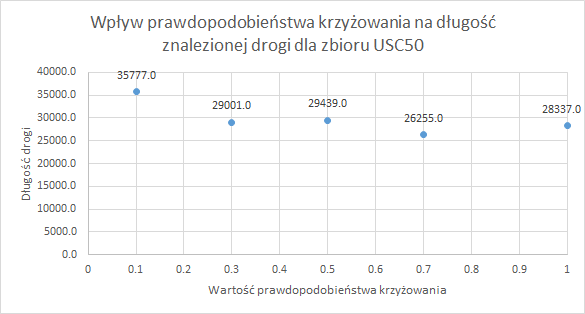
\includegraphics[scale=0.9]{IO_obrazy/excel_usca_kros}
\end{figure}


\begin{figure}[H]
\centering

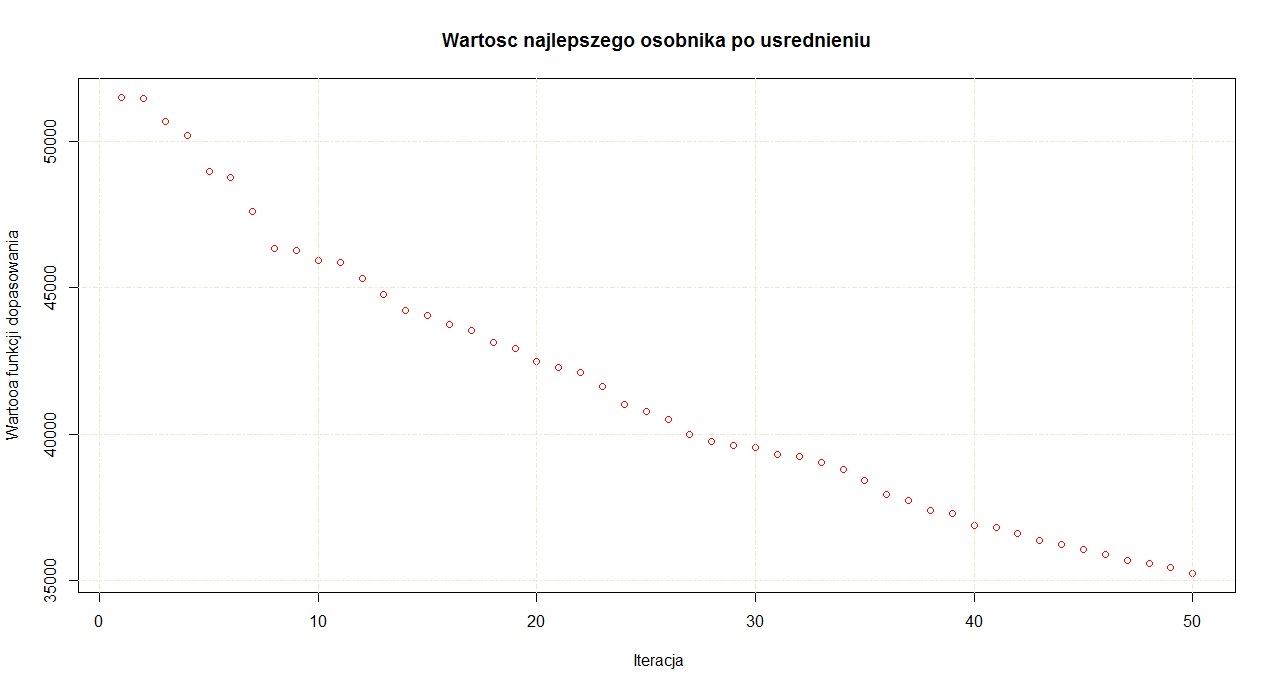
\includegraphics[scale=0.3]{IO_obrazy/US50_krz_01}
\caption{Wykres wartości najlepszego osobnika dla prawdopodobieństwa krzyżowania równe 0.1}
\end{figure}

\begin{figure}[H]
\centering

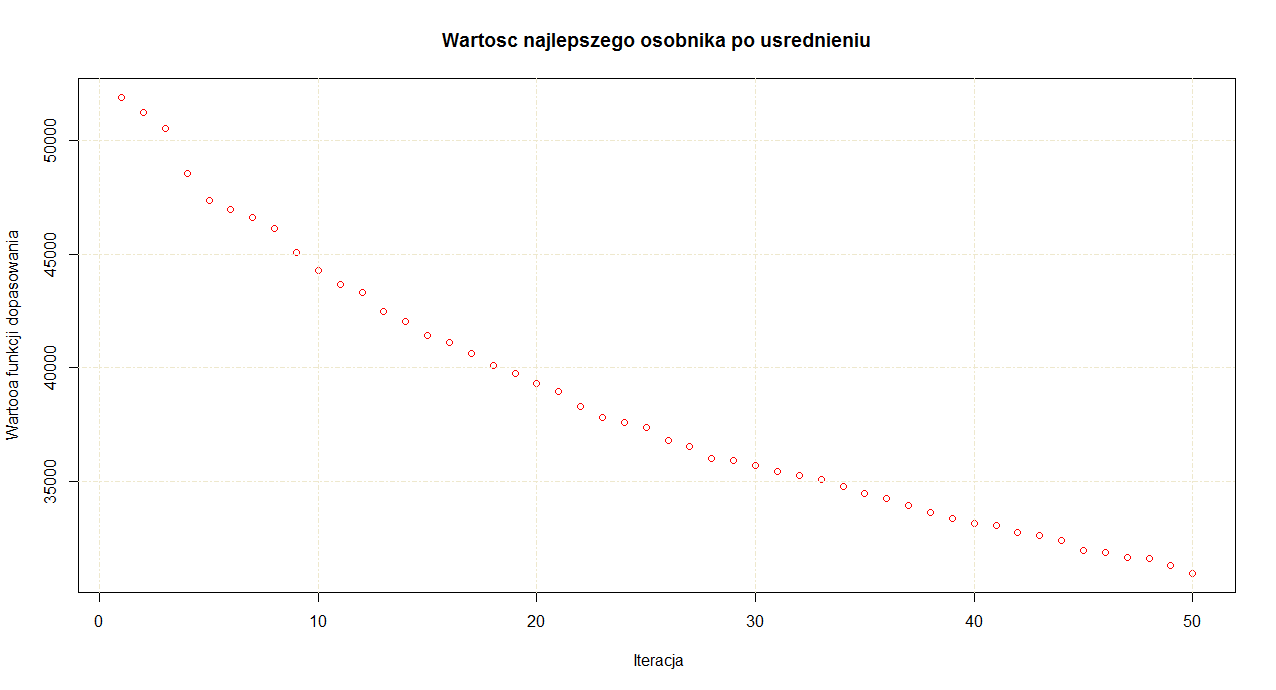
\includegraphics[scale=0.3]{IO_obrazy/US50_krz_03}
\caption{Wykres wartości najlepszego osobnika dla prawdopodobieństwa krzyżowania równe 0.3}
\end{figure}

\begin{figure}[H]
\centering

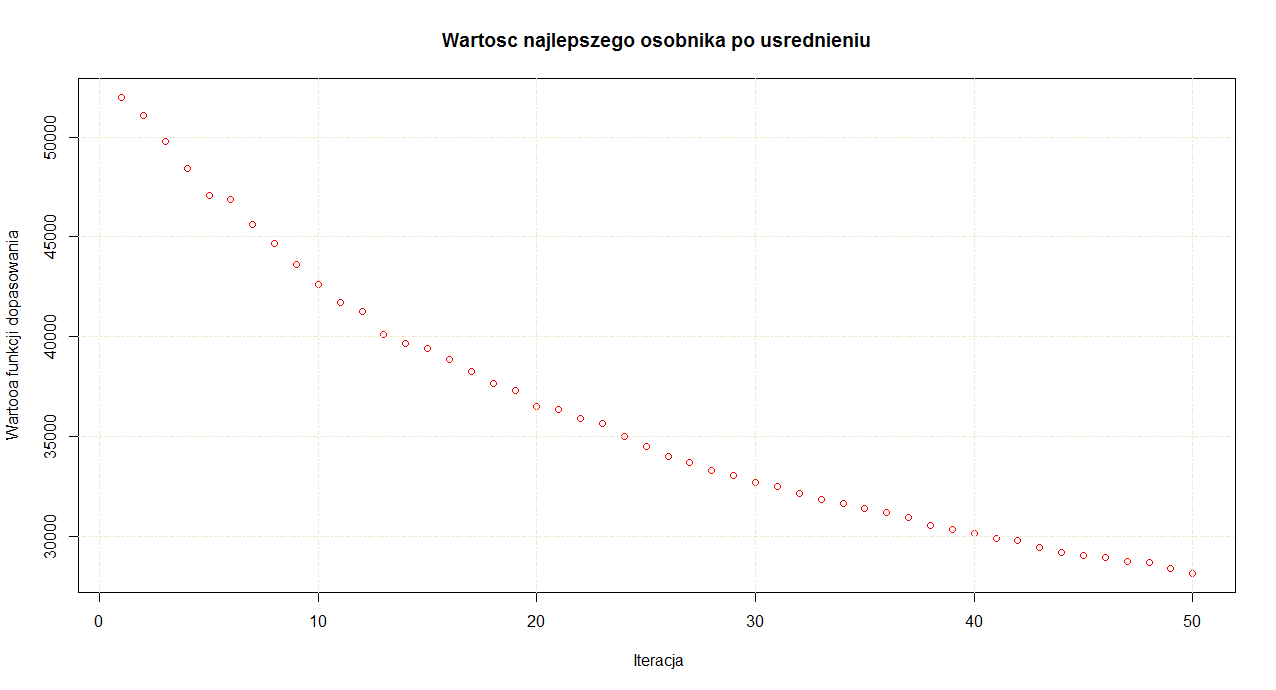
\includegraphics[scale=0.3]{IO_obrazy/US50_krz_07}
\caption{Wykres wartości najlepszego osobnika dla prawdopodobieństwa krzyżowania równe 0.7}
\end{figure}


\begin{figure}[H]
\centering

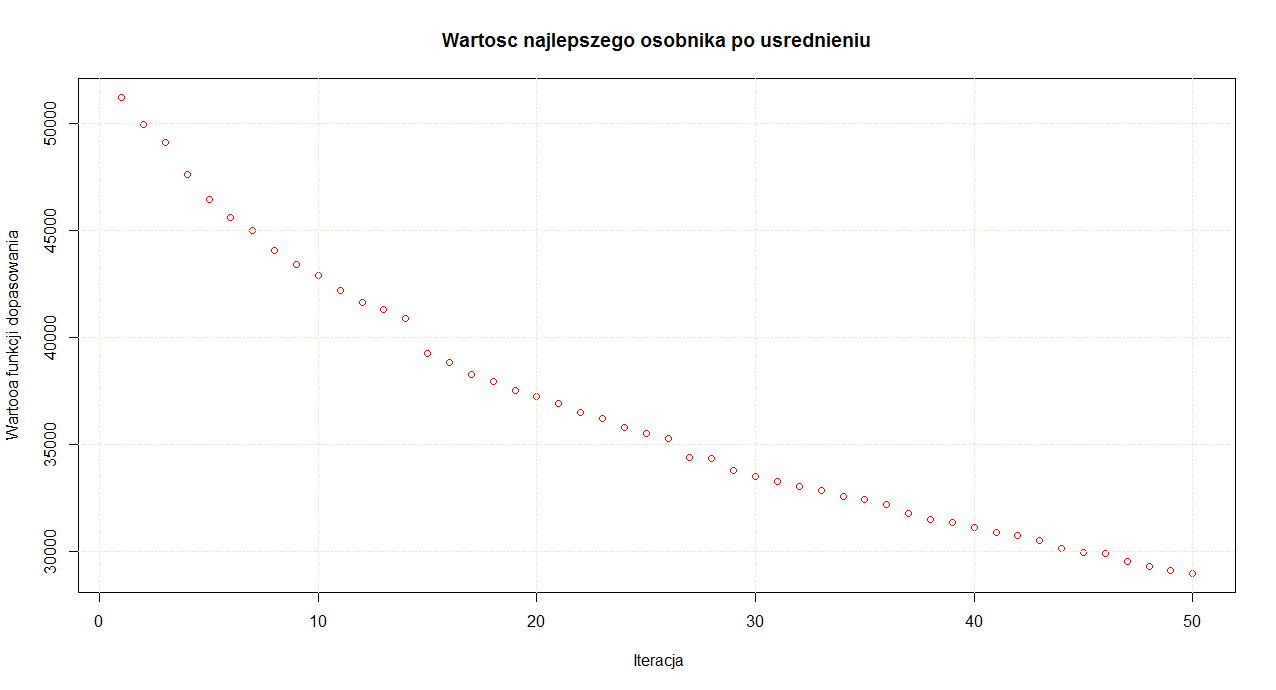
\includegraphics[scale=0.3]{IO_obrazy/US50_krz_1}
\caption{Wykres wartości najlepszego osobnika dla prawdopodobieństwa krzyżowania równe 1.0}
\end{figure}

Podsumowanie Najkrótsza droga została znaleziona dla prawdopodobieństwa krzyżowania równego 0.7. 



\newpage

\section{Mutacja}


\begin{figure}[H]
\centering

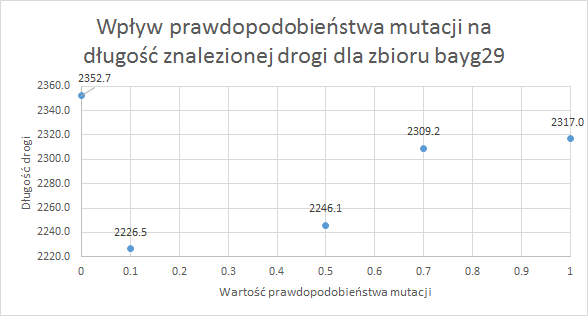
\includegraphics[scale=0.9]{IO_obrazy/excel_bayg29_mut}
\end{figure}

\begin{figure}[H]
\centering

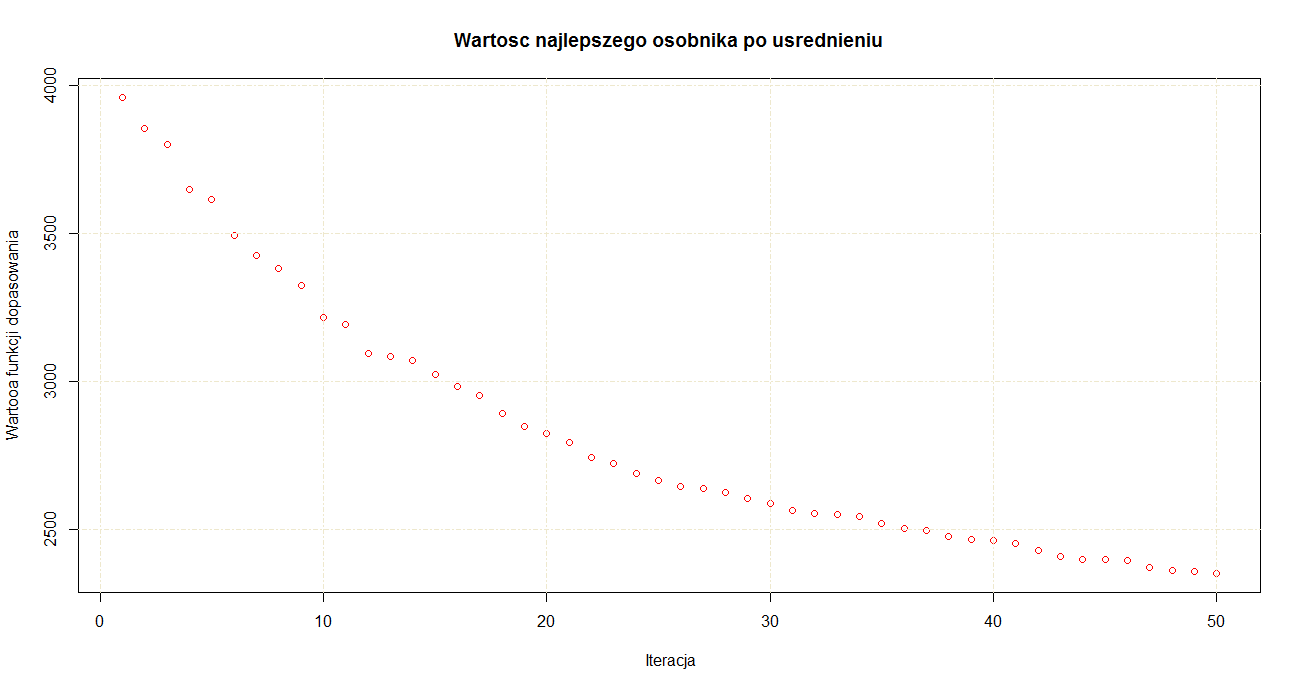
\includegraphics[scale=0.3]{IO_obrazy/bay29_mu_0}
\caption{Wykres wartości najlepszego osobnika dla prawdopodobieństwa mutacji równe 0}
\end{figure}

\begin{figure}[H]
\centering

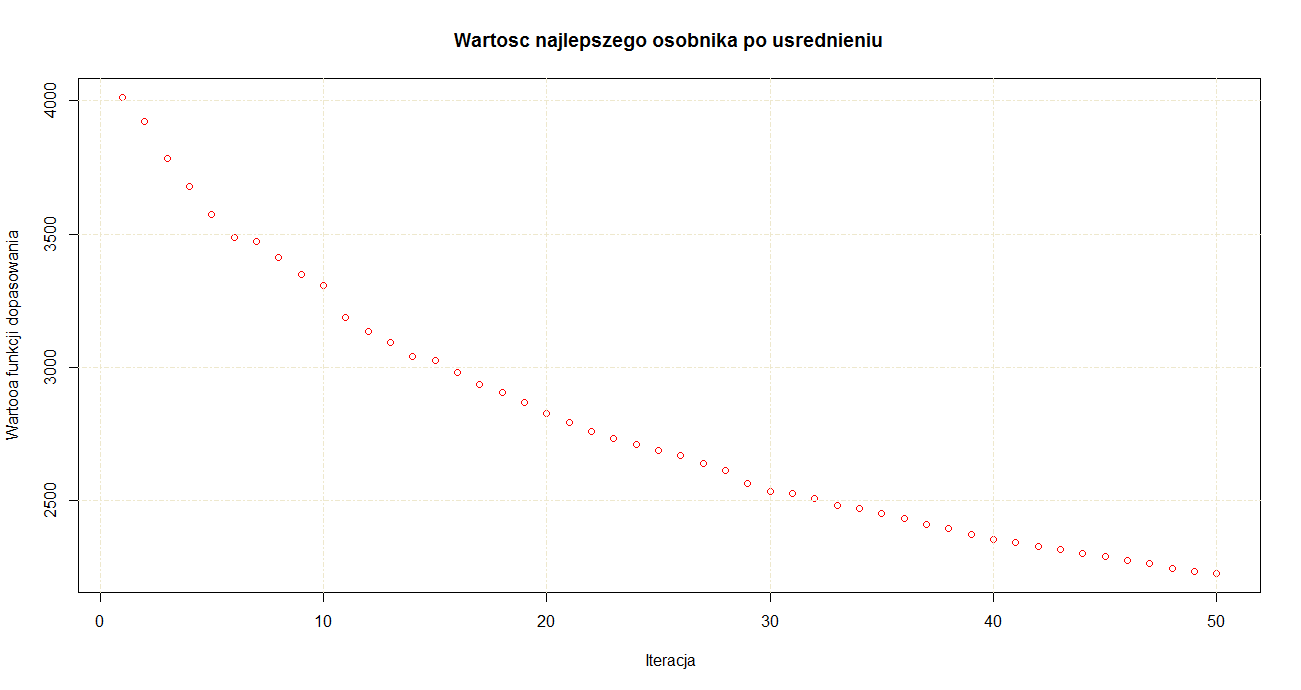
\includegraphics[scale=0.3]{IO_obrazy/bay29_mu_01}
\caption{Wykres wartości najlepszego osobnika dla prawdopodobieństwa mutacji równe 0.1}
\end{figure}

\begin{figure}[H]
\centering

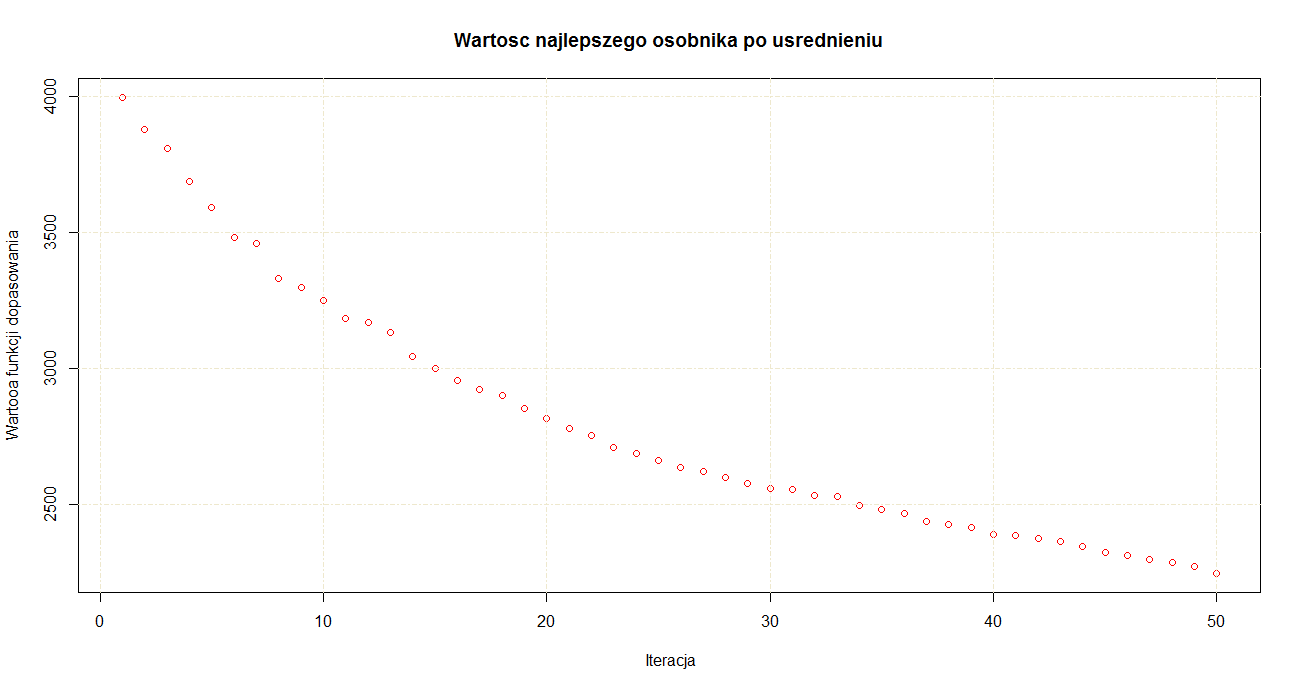
\includegraphics[scale=0.3]{IO_obrazy/bay29_mu_05}
\caption{Wykres wartości najlepszego osobnika dla prawdopodobieństwa mutacji równe 0.5}
\end{figure}

\begin{figure}[H]
\centering

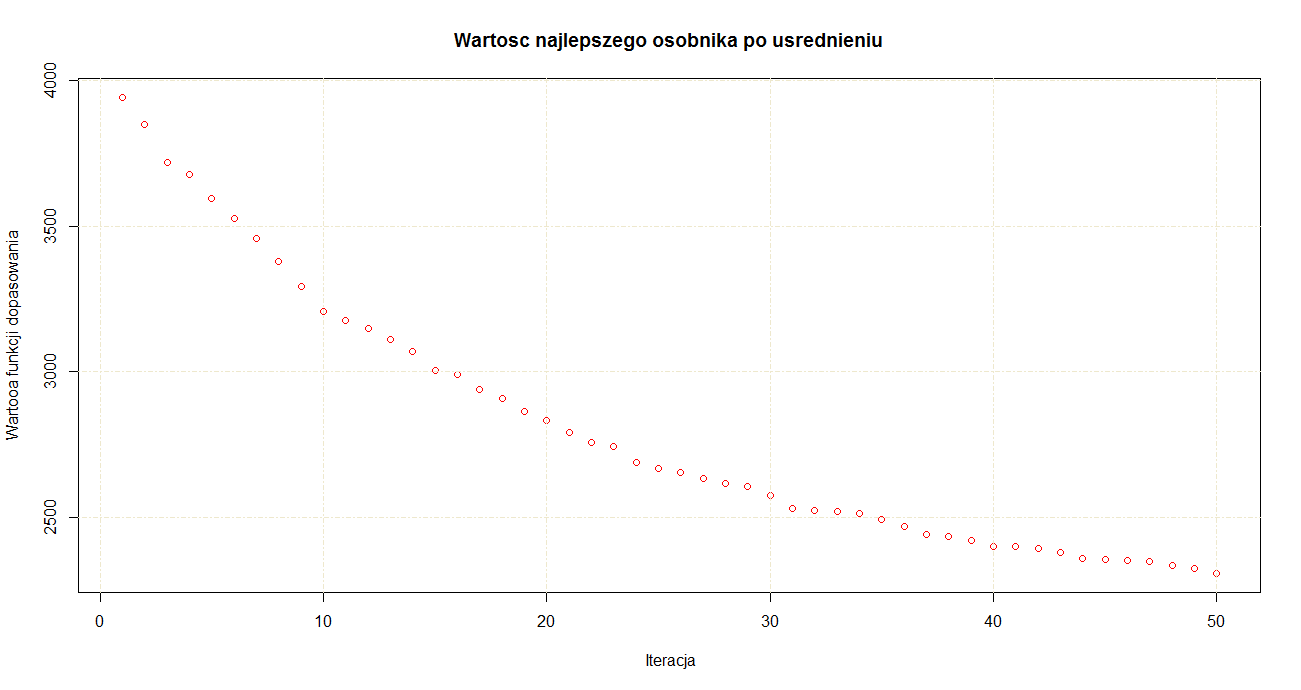
\includegraphics[scale=0.3]{IO_obrazy/bay29_mu_07}
\caption{Wykres wartości najlepszego osobnika dla prawdopodobieństwa mutacji równe 0.7}
\end{figure}


\begin{figure}[H]
\centering

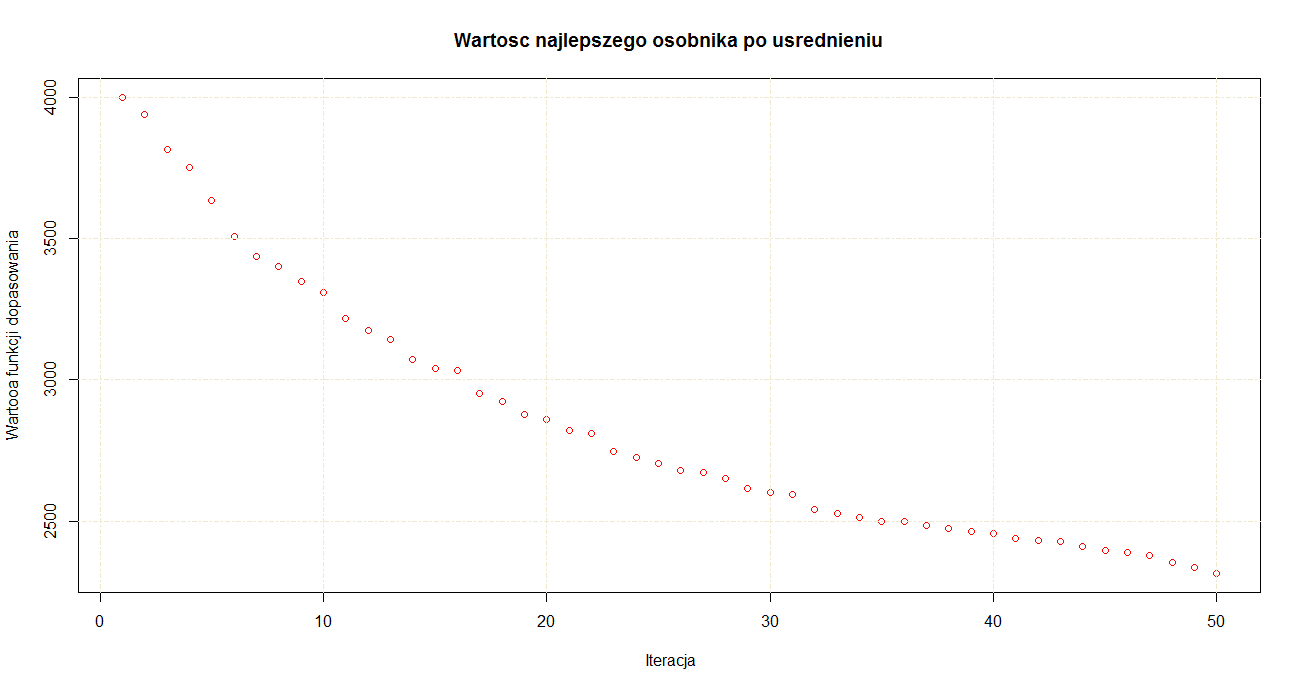
\includegraphics[scale=0.3]{IO_obrazy/bay29_mu_1}
\caption{Wykres wartości najlepszego osobnika dla prawdopodobieństwa krzyżowania równe 1}
\end{figure}

Podsumowanie Najkrótsza droga została znaleziona dla prawdopodobieństwa mutacji równego 0.1 - jest to jednocześnie wartość domyślna pakietu GA.


\newpage

\section{Elitaryzm}

\begin{figure}[H]
\centering

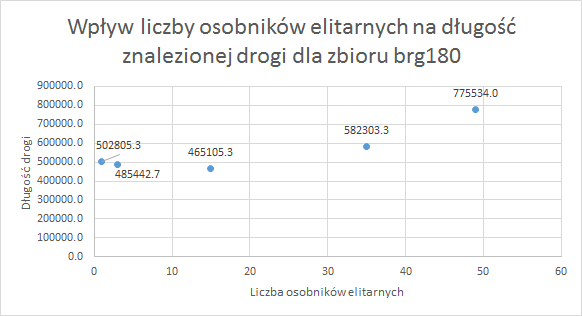
\includegraphics[scale=0.9]{IO_obrazy/excel_brg180_elit}
\end{figure}

\begin{figure}[H]
\centering

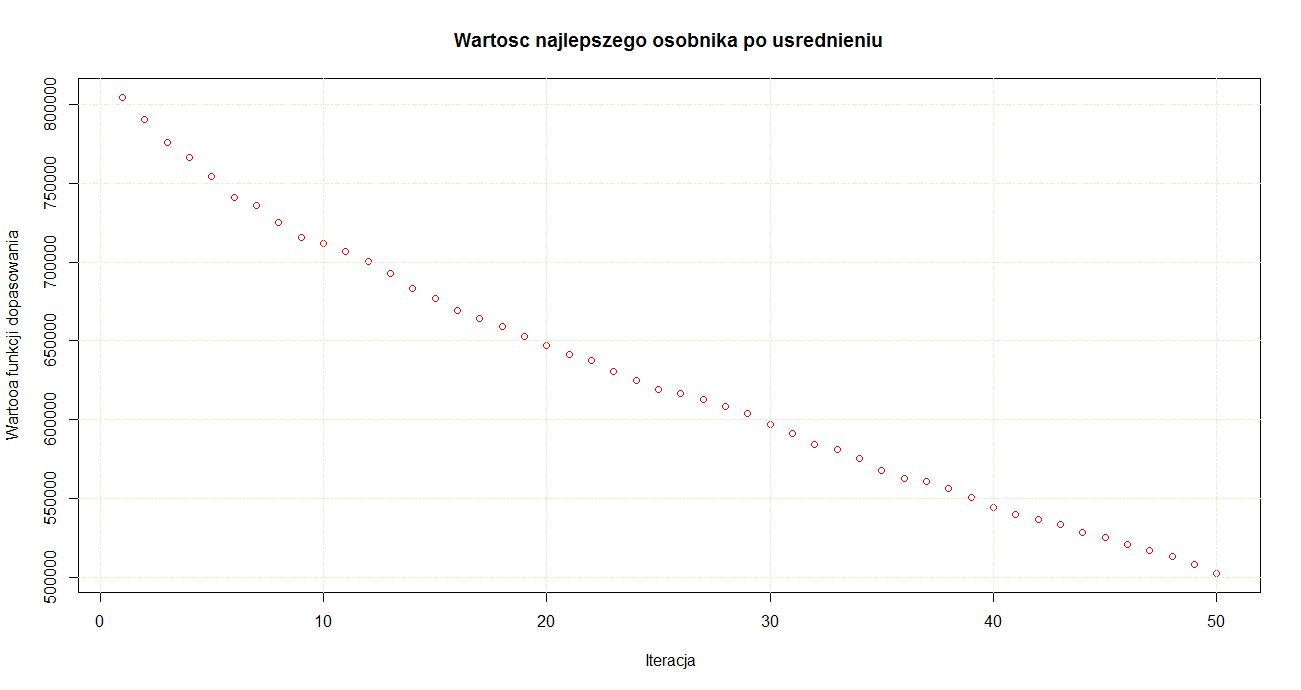
\includegraphics[scale=0.3]{IO_obrazy/brg180_elit_1}
\caption{Wykres wartości najlepszego osobnika dla liczby osobników elitarnych równych 1}
\end{figure}

\begin{figure}[H]
\centering

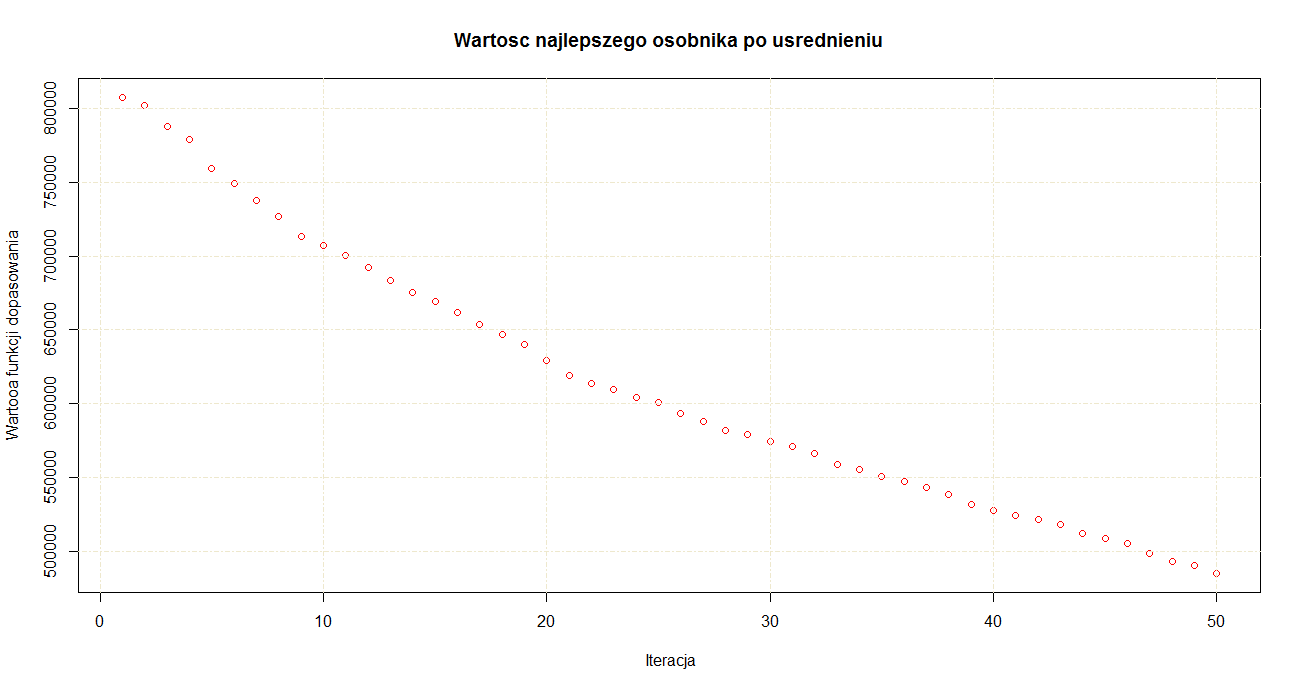
\includegraphics[scale=0.3]{IO_obrazy/brg180_elit_3}
\caption{Wykres wartości najlepszego osobnika dla liczby osobników elitarnych równych 3}
\end{figure}

\begin{figure}[H]
\centering

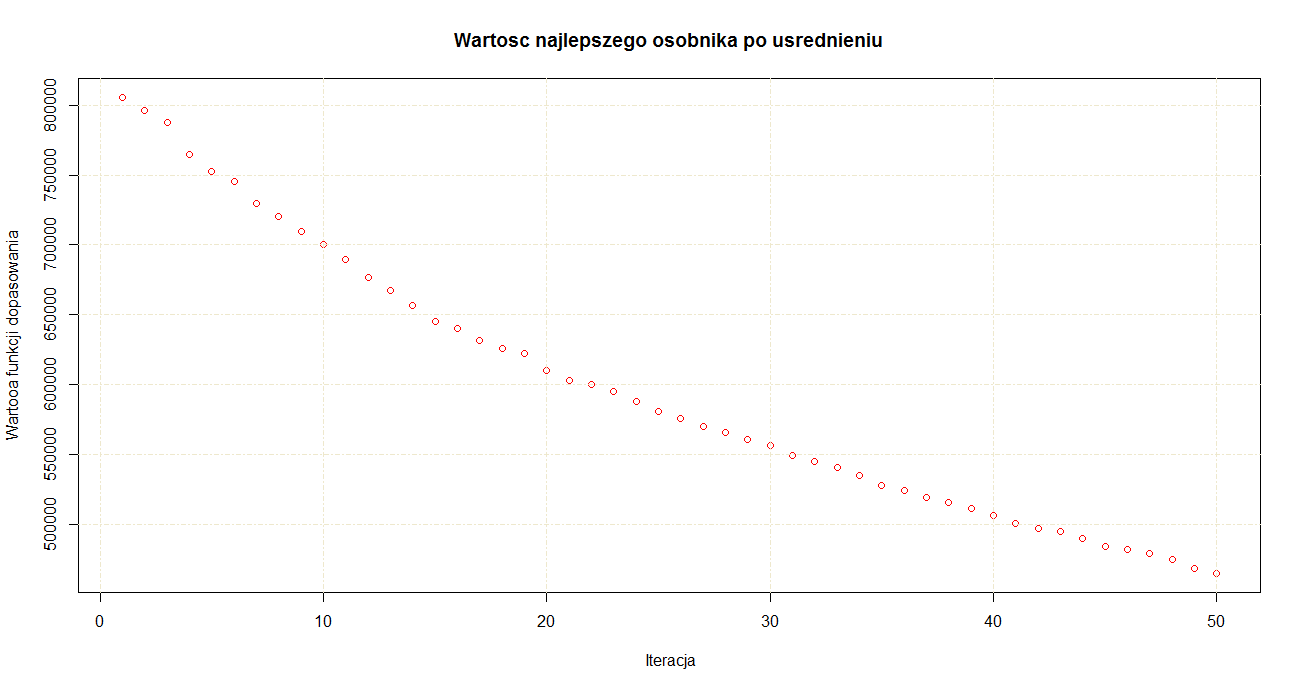
\includegraphics[scale=0.3]{IO_obrazy/brg180_elit_15}
\caption{Wykres wartości najlepszego osobnika dla liczby osobników elitarnych równych 15}
\end{figure}

\begin{figure}[H]
\centering

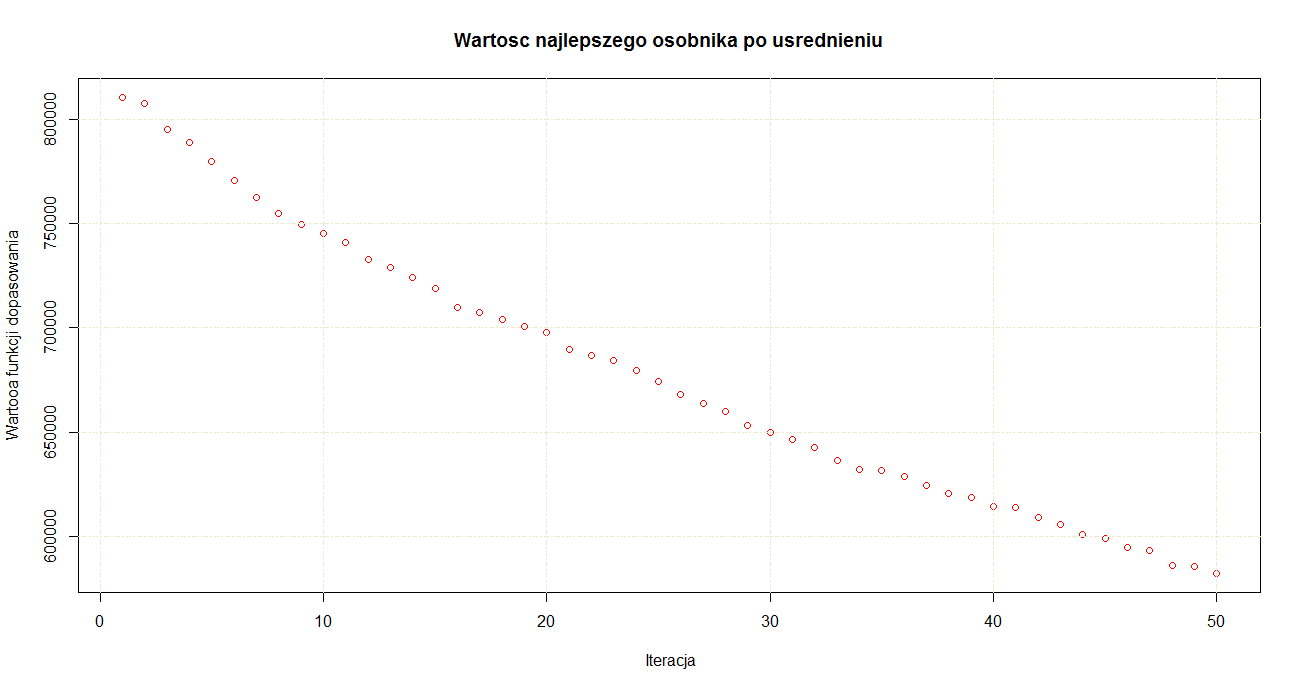
\includegraphics[scale=0.3]{IO_obrazy/brg180_elit_35}
\caption{Wykres wartości najlepszego osobnika dla liczby osobników elitarnych równych 35}
\end{figure}


\begin{figure}[H]
\centering

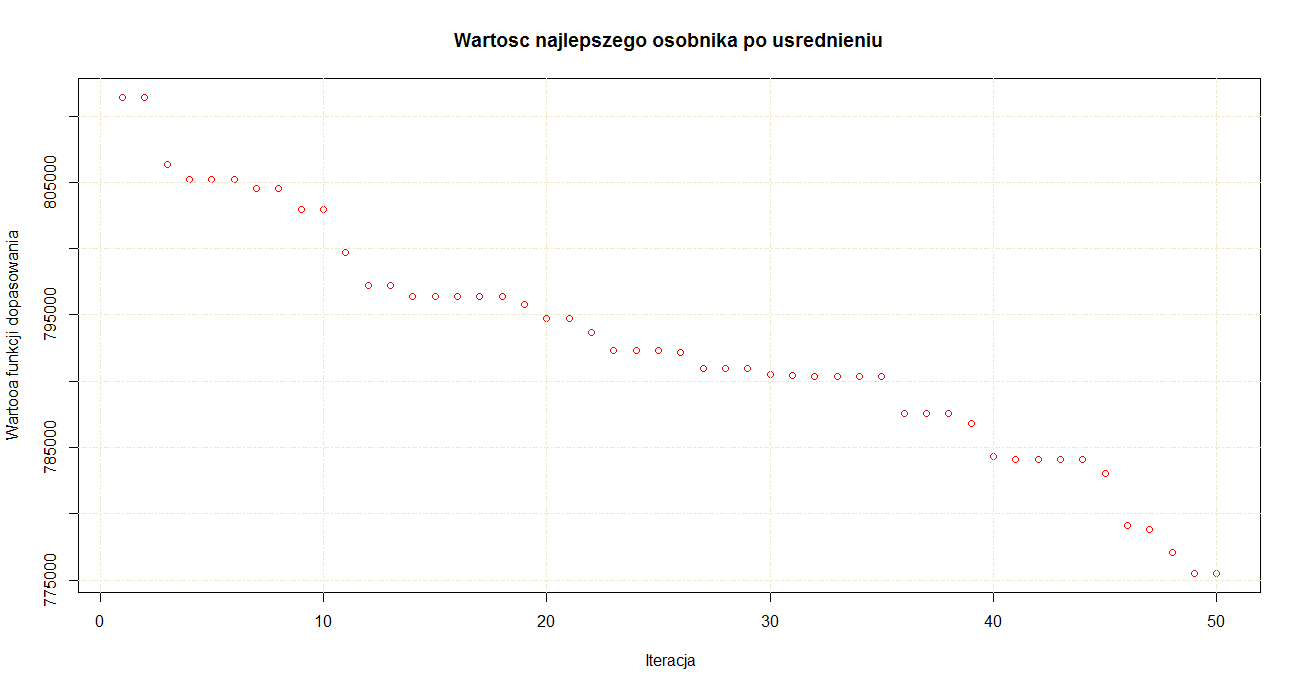
\includegraphics[scale=0.3]{IO_obrazy/brg180_elit_49}
\caption{Wykres wartości najlepszego osobnika dla liczby osobników elitarnych równych 49}
\end{figure}


Podsumowanie Najkrótsza droga została znaleziona gdy pozostawionych zostało 5 osobników elitarnych z populacji 50. 




\end{document}
Contact GitHub API Training Shop Blog About
© 2017 GitHub, Inc. Terms Privacy Security Status Help